\hypertarget{_alpha_of_k_8c}{
\section{/home/mgh/LanlGeoMag/libLanlGeoMag/AlphaOfK.c File Reference}
\label{_alpha_of_k_8c}\index{/home/mgh/LanlGeoMag/libLanlGeoMag/AlphaOfK.c@{/home/mgh/LanlGeoMag/libLanlGeoMag/AlphaOfK.c}}
}
{\tt \#include $<$stdio.h$>$}\par
{\tt \#include $<$math.h$>$}\par
{\tt \#include \char`\"{}Lgm/Lgm\_\-QuadPack.h\char`\"{}}\par
{\tt \#include \char`\"{}Lgm/Lgm\_\-MagModelInfo.h\char`\"{}}\par
{\tt \#include \char`\"{}Lgm/Lgm\_\-LstarInfo.h\char`\"{}}\par
{\tt \#include $<$gsl/gsl\_\-errno.h$>$}\par
{\tt \#include $<$gsl/gsl\_\-spline.h$>$}\par
{\tt \#include $<$string.h$>$}\par


Include dependency graph for AlphaOfK.c:\nopagebreak
\begin{figure}[H]
\begin{center}
\leavevmode
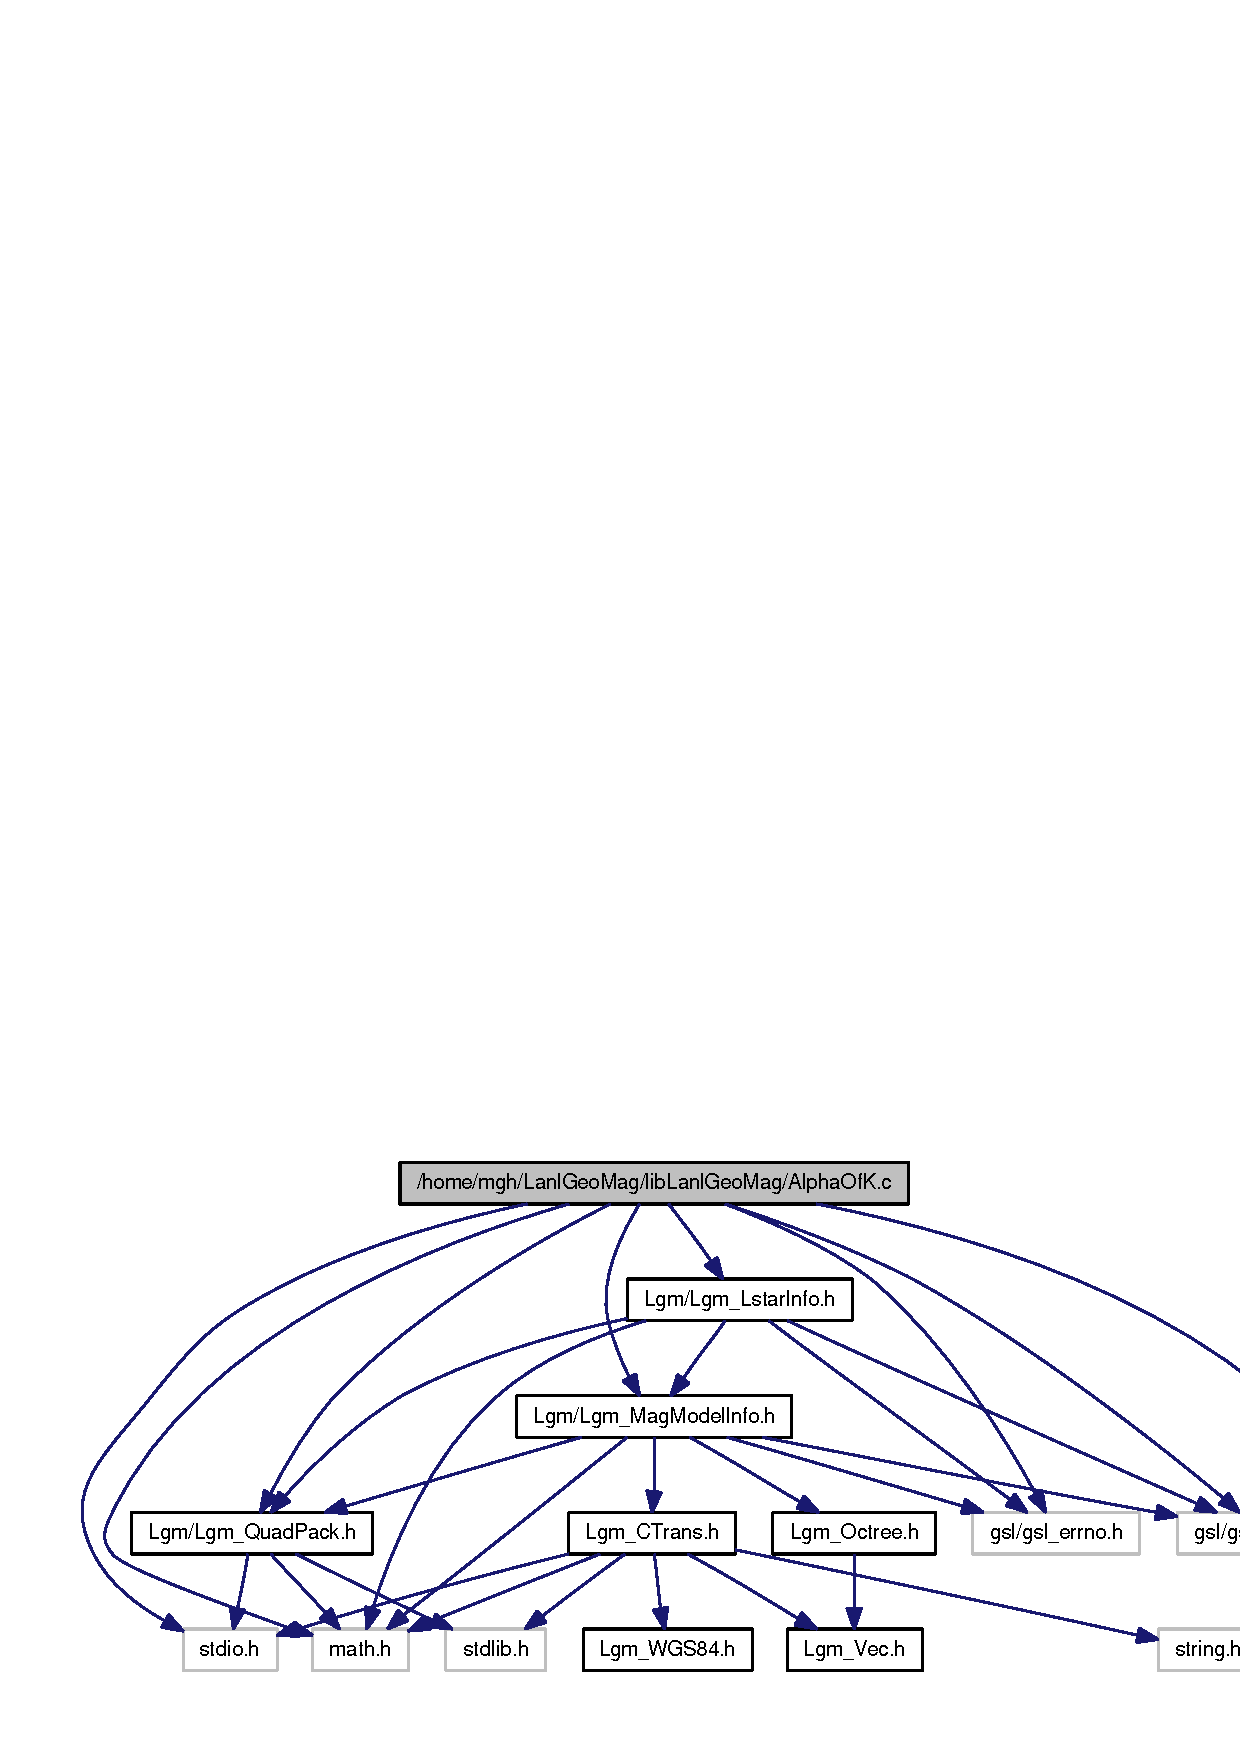
\includegraphics[width=331pt]{_alpha_of_k_8c__incl}
\end{center}
\end{figure}
\subsection*{Defines}
\begin{CompactItemize}
\item 
\#define \hyperlink{_alpha_of_k_8c_5ce702bb9d0edd19fbb1d576cfaf7010}{TRACE\_\-TOL}~1e-7
\item 
\#define \hyperlink{_alpha_of_k_8c_f468028083c9e52aa2c94ef3b9940450}{GOLD}~0.38197
\end{CompactItemize}
\subsection*{Functions}
\begin{CompactItemize}
\item 
double \hyperlink{_alpha_of_k_8c_8c0c461cb66bea86f5c7703017a24dde}{Func} (double Kt, double Alpha, \hyperlink{struct_lgm___lstar_info}{Lgm\_\-LstarInfo} $\ast$LstarInfo)
\item 
double \hyperlink{_alpha_of_k_8c_a9a43909d59850c622768267ce73421c}{AlphaOfK} (double K, \hyperlink{struct_lgm___lstar_info}{Lgm\_\-LstarInfo} $\ast$LstarInfo)
\end{CompactItemize}


\subsection{Define Documentation}
\hypertarget{_alpha_of_k_8c_5ce702bb9d0edd19fbb1d576cfaf7010}{
\index{AlphaOfK.c@{AlphaOfK.c}!TRACE\_\-TOL@{TRACE\_\-TOL}}
\index{TRACE\_\-TOL@{TRACE\_\-TOL}!AlphaOfK.c@{AlphaOfK.c}}
\subsubsection[{TRACE\_\-TOL}]{\setlength{\rightskip}{0pt plus 5cm}\#define TRACE\_\-TOL~1e-7}}
\label{_alpha_of_k_8c_5ce702bb9d0edd19fbb1d576cfaf7010}




Definition at line 10 of file AlphaOfK.c.\hypertarget{_alpha_of_k_8c_f468028083c9e52aa2c94ef3b9940450}{
\index{AlphaOfK.c@{AlphaOfK.c}!GOLD@{GOLD}}
\index{GOLD@{GOLD}!AlphaOfK.c@{AlphaOfK.c}}
\subsubsection[{GOLD}]{\setlength{\rightskip}{0pt plus 5cm}\#define GOLD~0.38197}}
\label{_alpha_of_k_8c_f468028083c9e52aa2c94ef3b9940450}




Definition at line 11 of file AlphaOfK.c.

\subsection{Function Documentation}
\hypertarget{_alpha_of_k_8c_8c0c461cb66bea86f5c7703017a24dde}{
\index{AlphaOfK.c@{AlphaOfK.c}!Func@{Func}}
\index{Func@{Func}!AlphaOfK.c@{AlphaOfK.c}}
\subsubsection[{Func}]{\setlength{\rightskip}{0pt plus 5cm}double Func (double {\em Kt}, \/  double {\em Alpha}, \/  {\bf Lgm\_\-LstarInfo} $\ast$ {\em LstarInfo})}}
\label{_alpha_of_k_8c_8c0c461cb66bea86f5c7703017a24dde}




Definition at line 109 of file AlphaOfK.c.

Here is the call graph for this function:\nopagebreak
\begin{figure}[H]
\begin{center}
\leavevmode
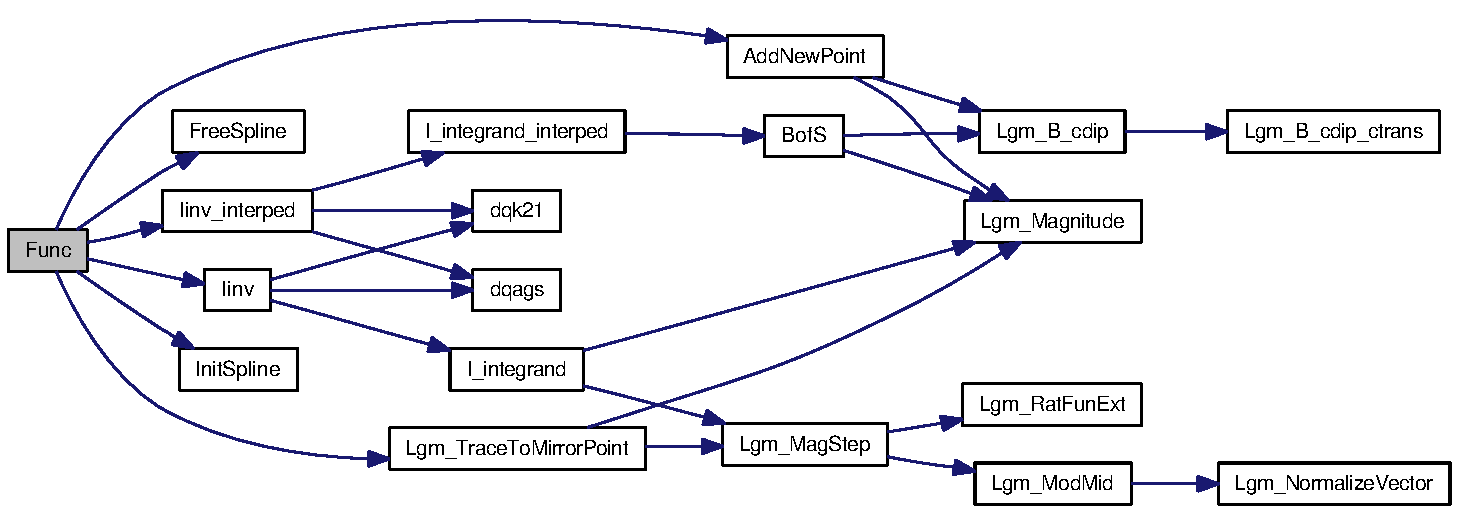
\includegraphics[width=368pt]{_alpha_of_k_8c_8c0c461cb66bea86f5c7703017a24dde_cgraph}
\end{center}
\end{figure}


Here is the caller graph for this function:\nopagebreak
\begin{figure}[H]
\begin{center}
\leavevmode
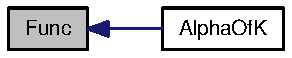
\includegraphics[width=88pt]{_alpha_of_k_8c_8c0c461cb66bea86f5c7703017a24dde_icgraph}
\end{center}
\end{figure}
\hypertarget{_alpha_of_k_8c_a9a43909d59850c622768267ce73421c}{
\index{AlphaOfK.c@{AlphaOfK.c}!AlphaOfK@{AlphaOfK}}
\index{AlphaOfK@{AlphaOfK}!AlphaOfK.c@{AlphaOfK.c}}
\subsubsection[{AlphaOfK}]{\setlength{\rightskip}{0pt plus 5cm}double AlphaOfK (double {\em K}, \/  {\bf Lgm\_\-LstarInfo} $\ast$ {\em LstarInfo})}}
\label{_alpha_of_k_8c_a9a43909d59850c622768267ce73421c}




Definition at line 24 of file AlphaOfK.c.

Here is the call graph for this function:\nopagebreak
\begin{figure}[H]
\begin{center}
\leavevmode
\includegraphics[width=415pt]{_alpha_of_k_8c_a9a43909d59850c622768267ce73421c_cgraph}
\end{center}
\end{figure}
